\documentclass[a4paper,11pt]{scrreprt}

\usepackage[ngerman]{babel}
\usepackage[utf8]{inputenc}
\usepackage{amsthm}
\usepackage{enumerate}
\usepackage{mathtools}
\usepackage{amssymb}
\usepackage{stmaryrd}
\usepackage{listings}
\usepackage[dvipsnames]{xcolor}
\usepackage{hyperref}

\usepackage[headsepline]{scrlayer-scrpage}
\pagestyle{scrheadings}
\clearscrheadfoot
\ohead{Elisa Junghans\\Mirko Dransfeld}
\ihead{Wissenschaftliches Rechnen\\SS 19}
\chead{Praktikum MatLab\\Rubik's Cube}
\cfoot*{\pagemark}

\title{Rubik's Cube}
\subtitle{MatLab Praktikum}
\author{Elisa Junghans\and Mirko Dransfeld}
\date{}

\setcounter{secnumdepth}{4}

\hypersetup{
    unicode=true,
    colorlinks=true,
    linkcolor=Magenta,
    linktoc=all,
    citecolor=NavyBlue,
    filecolor=NavyBlue,
    urlcolor=NavyBlue,
    final=true
}

\lstset{ %
    basicstyle=\small\ttfamily,
    language=Matlab,
    showtabs=false,
    tabsize=2,
    captionpos=t,
    breaklines=true,
    extendedchars=true,
    showstringspaces=false,
    flexiblecolumns=true,
    numbers=left,
    numbersep=8pt,
    stepnumber=1,
    numberstyle=\color{Gray},
    keywordstyle=\color{Blue},
    commentstyle=\color{ForestGreen}
}

\newcommand{\codeimport}[4][0]{
  \lstinputlisting[firstnumber=#2,tabsize=4,framexleftmargin=\the\dimexpr -18pt * #1\relax,numbersep=\the\dimexpr \the\dimexpr -18pt * #1\relax + 8pt\relax,xleftmargin=\the\dimexpr -18pt * #1\relax, linerange={#2-#3}]{#4}
}

\newcommand{\coderef}[1]{
  \texttt{\nameref{#1}}
}
\newcommand{\codeinline}[1]{
  \lstinline!#1!
}
\newcommand{\codecustomref}[2]{
  \hyperref[#2]{\lstinline!#1!}
}


\newcommand{\chap}[2]{
  \chapter{#1}\label{#2}
}
\renewcommand{\sec}[2]{
  \section{#1}\label{#2}
}
\newcommand{\subsec}[2]{
  \subsection{#1}\label{#2}
}
\newcommand{\subsubsec}[2]{
  \subsubsection{#1}\label{#2}
}

%%
%%
%%
%%  Hallo Elisa :)
%%
%%
%%
%%  Überschriften sind: (absteigende Wichtigkeit)
%%  \chap{}{}       Kapitel
%%  \sec{}{}        sektion   (ist das ein wort?)
%%  \subsec{}{}     untersektion
%%  \subsubsec{}{}  unteruntersektion
%%
%%  alle funktionieren mit z.B. \chap{<Überschrift>}{<Labelname>}
%%  Die Labelnamen sind dafür um später auf die Funktion verweisen zu können, siehe \coderef
%%  Wichtig: Unterstriche in den Überschrifter escapen mit \_ !
%%
%%
%%
%%  wenn du Code aus einer Datei einbinden willst: \codeimport{<Anfang>}{<Ende>}{<Datei>}
%%  z.B.  \codeimport{44}{49}{RubiksCube}  fügt Zeilen 44-49 aus RubiksCube.m ein
%%
%%  wenn du eine bestimmte Funktion referenzieren willst: \coderef{<Labelname>}
%%  z.B.  \coderef{sec:figure}  macht daraus figure() mit einem Verweis zu \sec{figure()}{figure}. (es setzt den Funktionsnamen ein, so wie du ihn benannt hast)
%%
%%  wenn du einen kleinen inline-codeteil haben willst: \codeinline{<Text>}
%%  z.B.  \codeinline{figure(Option1, Wert1, ...)}  schreibt den <Text> als Code (inline)
%%
%%
%%
%%  Kannst dir ja das angucken was ich bisher geschrieben habe. Bei Problemen oder Feature-Wünschen -> Hey :)
%%
%%
%%

\begin{document}
  \maketitle

  \chap{Aufbau des Programms}{aufbau}
    \sec{RubiksCube.m}{rubikscube}
      \subsec{Variablen}{variablen}
        \subsubsec{face\_colors}{facecolors}
          Dies ist ein zweidimensionales Array, dass die Farben der einzelnen Flächen des Würfels speichert. Dabei entsprechen die Zahlen 1--6 den Seiten des Würfels, deren Farbe die Flächen haben. Die erste Koordinate ist die Seiten- und die Zweite die Flächennummer auf der jeweiligen Seite. \codeinline{face_colors(3,5)} wäre dementsprechend Fläche 5 auf Seite 3 (blau, unten rechts).
          \begin{figure}[!h]
            \centering
            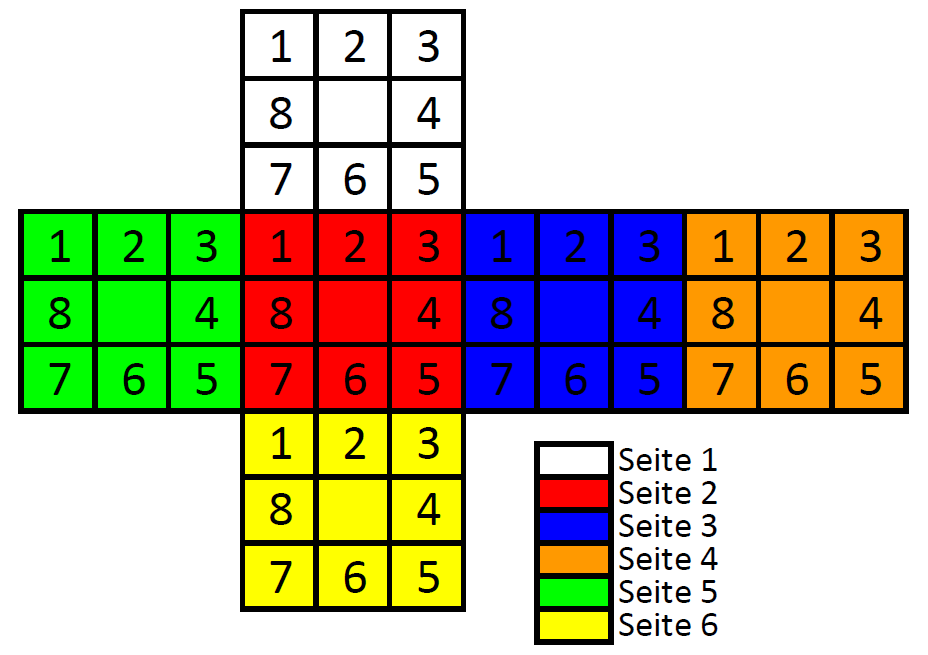
\includegraphics[width=0.5\columnwidth]{cubeMapCropped}
            \caption{Position der Flächen in \coderef{facecolors}}
          \end{figure}\newline
          Die Mittelflächen müssen hierbei nicht beachtet werden, da man ihre Position nicht durch Drehungen verändern kann. (siehe \autoref{grundlagen} \nameref{grundlagen})

      \subsec{Funktionen}{funktionen}
        \subsubsec{load\_presets()}{loadpresets}
          Diese Funktion interagiert mit der Datei \coderef{resources} und lädt sowohl die Farbdefinitionen für die Custom-Farbe, als auch die Presets in die Variablen \codeinline{color_dialog_colors} beziehungsweise \codeinline{cube_presets}. Die Datei wird mithlife der Funktion \codeinline{fgetl()} zeilenweise ohne newline-Zeichen ausgelesen. Dann werden mithlife von \codeinline{regexp()} die entsprechenden Teile extrahiert.

          Im folgenden Beispiel wird die erste Zeile zu Beginn in ein cell-Array  aus je sechs hex-Zeichen aufgeteilt und dann mithilfe von \coderef{hex2rgb} in ein Array von RGB-Farben umgewandelt.
          \codeimport[3]{136}{137}{RubiksCube.m}

        \subsubsec{hex2rgb()}{hex2rgb}
          Diese Funktion wandelt ein cell-Array in ein Array von RGB-Farben um. Da RGB-Farben aus drei Komponenten bestehen, ist der Rückgabewert dieser Funktion ein zweidimensionales Array, bei dem man mit dem ersten Parameter die Farbe wählt und mit dem Zweiten auf die jeweiligen RGB-Komponenten zugreifen kann.

        \subsubsec{ui\_setup()}{uisetup}
          In dieser Funktion werden mithilfe von \coderef{uimenu} die Menüleiste angelegt und mit \coderef{uicontrol} die Elemente auf dem UI erzeugt. Außerdem werden die Achsen der Figur sowohl \codeinline{off} als auch \codeinline{equal} gesetzt und \coderef{generatecenterpieces}, \coderef{rotateview}, sowie \coderef{loadpresets} aufgerufen.

        \subsubsec{rotate\_view}{rotateview}
          Diese Funktion rotiert die Figur in die Ausgangsposition mithilfe von: \codeimport[1]{377}{379}{RubiksCube.m}

        \subsubsec{generate\_centerpieces()}{generatecenterpieces}
          Mit \coderef{patch} werden die Mitten der Seiten erzeugt. Da diese durch die Drehungen nicht verändert werden können, sind diese nicht in \coderef{facecolors} enthalten.

        \subsubsec{solve\_cube()}{solvecube}

    \sec{turn.m}{turn}
      Diese Datei beinhaltet die Funktionen zum Drehen des Würfels. Dazu werden die Elemente von \codeinline{cube} je nach Drehung vertauscht. Diese Drehung wird durch \codeinline{dir} bestimmt. Der Aufbau von \codeinline{cube} entspricht dem der \coderef{facecolors}. \codeinline{dir} ist eine Zahl von 1--12. In einem \codeinline{switch}-Statement wird dann die jeweilige Rotation (siehe \autoref{grundlagen} \nameref{grundlagen}).

    \sec{generate\_solution.m}{generatesolution}

    \sec{f2l\_recursive.m}{f2lrecursive}

    \sec{resources.txt}{resources}
      In der ersten Zeile werden, wenn festgelegt, die RGB-Farben für die Custom-Farboption in der Reihenfolge Top-Front-Right-Back-Left-Bottom definiert. Alle weiteren Zeilen beinhalten die Presets mit zugehörigem Namen. Bei Programmstart wird diese Datei in der Funktion \coderef{loadpresets} geladen.

  \chap{Lösungsalgorithmus}{algorithm}
    \sec{Grundlagen}{grundlagen}

    \sec{untere und mittlere Ebene}{f2l}

    \sec{obere Ebene}{oben}

    \sec{rekursiver Ansatz}{recursive}

  \chap{Besondere MatLab-Funktionen}{matlab}
    \sec{figure()}{figure}

    \sec{patch()}{patch}

    \sec{uicontrol()}{uicontrol}

    \sec{uimenu()}{uimenu}

    \sec{dialog()}{dialog}

\end{document}
